%==============================================================================
% Sjabloon poster bachproef
%==============================================================================
\documentclass[a0,portrait]{hogent-poster}

% Info over de opleiding
\course{Bachelorproef}
\studyprogramme{toegepaste informatica}
\academicyear{2025-2026}
\institution{Hogeschool Gent, Valentin Vaerwyckweg 1, 9000 Gent}

% Info over de bachelorproef
\title{Automatische detectie van misinformatie op Mastodon}
\subtitle{Vergelijking van machine learning modellen}
\author{Kyanu Neckebroek}
\email{kyanu.neckebroek@student.hogent.be}
\supervisor{S. Van Impe}
\cosupervisor{K. Cools}

\specialisation{Toegepaste Informatica}
\keywords{misinformatie, machine learning, BERT, Mastodon, decentrale netwerken}
\projectrepo{https://github.com/HoGentTIN/latex-hogent-bachproef}

% Extra pakketten voor de layout
\usepackage{pgfplots}
\pgfplotsset{compat=1.17}
\usepackage[most]{tcolorbox}
\usepackage{tikz}
\usetikzlibrary{shapes.geometric, arrows.meta, positioning, fit, backgrounds}

% Kleuren
\definecolor{hogent-blue}{HTML}{0075b3} % Officiële HOGENT blauw
\definecolor{html-gray-bg}{HTML}{f1f5f9}
\definecolor{html-gray-border}{HTML}{cbd5e1}
\definecolor{html-gray-text}{HTML}{475569}

% Commando voor HTML-stijl sectietitels
\newcommand{\htmlsection}[1]{
    \vspace{1.5cm}
    \noindent{\Large\bfseries\sffamily\color{hogent-blue}\MakeUppercase{#1}}\\[-0.5ex]
    {\color{hogent-blue}\rule{\linewidth}{3pt}}\vspace{1.5ex}
}

% Commando voor tags
\newcommand{\htmltag}[1]{%
    \tikz[baseline=(X.base)] \node[draw=html-gray-border, fill=html-gray-bg, text=html-gray-text, rounded corners=4pt, inner sep=6pt, font=\large] (X) {#1};%
}

% Stijl voor Result Cards
\newtcolorbox{resultcard}[1][]{
    enhanced,
    colback=html-gray-bg,
    colframe=html-gray-border,
    boxrule=2pt,
    arc=8pt,
    halign=center,
    valign=center,
    #1
}

% Spacing en layout optimalisatie
\setlength{\columnsep}{60pt}
\renewcommand{\columnseprule}{0pt}

\begin{document}

\maketitle

\vspace{1.5cm}

% --- START KOLOMMEN ---
\begin{multicols}{2}

% ================= KOLOM 1 =================
\htmlsection{Introductie \& Probleemstelling}

Mastodon groeit als \textbf{gedecentraliseerd} sociaal netwerk zonder centrale moderatie. Bestaande misinformatiedetectiemodellen zijn gebouwd voor platforms als Twitter en presteren suboptimaal op de heterogene Mastodon-data (max. 500 tekens, wisselende metadata).

\vspace{12pt}
\noindent\textbf{Hoofdonderzoeksvraag:}\\
\textit{Welke machine learning modellen zijn het meest geschikt voor het detecteren van misinformatie op Mastodon en welke inhoudelijke factoren beïnvloeden de nauwkeurigheid van deze modellen?}

\vspace{8pt}
\noindent\textbf{Deelvragen:}
\begin{itemize}
\item Wat is de relatieve prestatie van BERT versus traditionele modellen (SVM, Logistic Regression)?
\item Welke factoren (berichtlengte, bronbetrouwbaarheid, taalgebruik) hebben statistisch significante invloed?
\item Hoe generaliseren modellen van de LIAR-dataset naar Mastodon-specifieke berichten?
\end{itemize}

\htmlsection{Methodologie}

\begin{itemize}
    \item \textbf{Data:} LIAR (12.836 claims) + 300 handmatig gelabelde Mastodon-berichten. Binaire classificatie: \textit{waar} vs. \textit{onwaar}.
    \item \textbf{Modellen:} SVM (TF-IDF), Logistic Regression (TF-IDF), en BERT (fine-tuned). Alle getraind met vaste seed.
    \item \textbf{Evaluatie:} F1-score (macro), Precision, Recall, AUC-ROC en factoranalyse (ANOVA, Chi-kwadraat, Mann-Whitney U).
\end{itemize}

\vspace{16pt}
\noindent
\htmltag{Mastodon} \htmltag{LIAR-Dataset} \htmltag{BERT} \htmltag{Fediverse} \htmltag{Macro F1-score}

\vspace{1.5cm}
\begin{center}
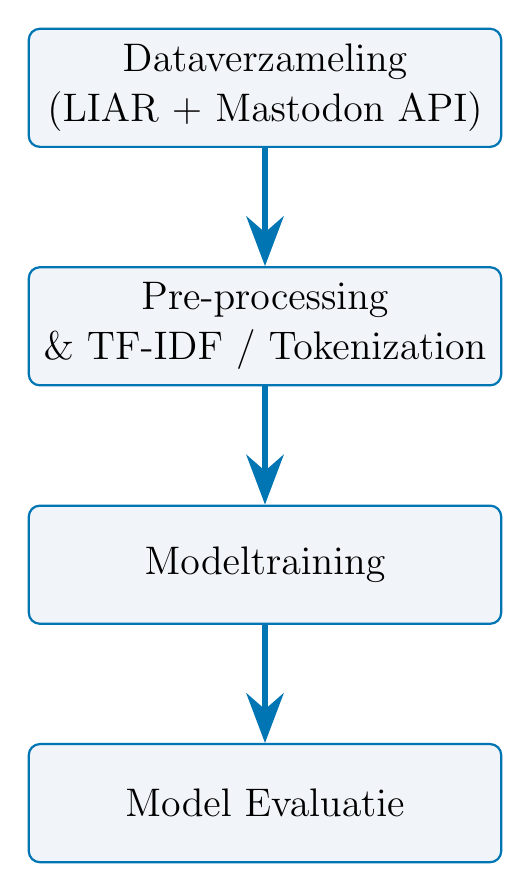
\begin{tikzpicture}[
    node distance=1.5cm and 1cm,
    box/.style={draw=hogent-blue, thick, rounded corners, fill=html-gray-bg, align=center, minimum width=6cm, minimum height=1.5cm, font=\Large},
    arrow/.style={-{Stealth[scale=1.5]}, line width=2pt, hogent-blue}
]
    \node[box] (data) {Dataverzameling\\(LIAR + Mastodon API)};
    \node[box, below=of data] (prep) {Pre-processing\\\& TF-IDF / Tokenization};
    \node[box, below=of prep] (train) {Modeltraining};
    \node[box, below=of train] (eval) {Model Evaluatie};
    
    \draw[arrow] (data) -- (prep);
    \draw[arrow] (prep) -- (train);
    \draw[arrow] (train) -- (eval);
\end{tikzpicture}
\vspace{15pt}
\\
\footnotesize \textcolor{html-gray-text}{Figuur 1: Dataverzameling- en trainingspipeline}
\end{center}

\vfill\null
\columnbreak
% ================= KOLOM 2 =================

\htmlsection{Resultaten}

% 2x2 Grid voor resultaten
\noindent
\begin{minipage}{0.48\linewidth}
    \begin{resultcard}[colframe=hogent-blue, boxrule=3pt] % Beste model benadrukt
        \vspace{10pt}
        \Large\textbf{\textcolor{hogent-blue}{BERT}}\\[5pt]
        \Huge\textbf{\textcolor{hogent-blue}{0.638}}\\[5pt]
        \normalsize \textcolor{html-gray-text}{MACRO F1}
        \vspace{10pt}
    \end{resultcard}
\end{minipage}\hfill
\begin{minipage}{0.48\linewidth}
    \begin{resultcard}
        \vspace{10pt}
        \Large\textbf{\textcolor{html-gray-text}{LOG. REGRESSION}}\\[5pt]
        \Huge\textbf{0.633}\\[5pt]
        \normalsize \textcolor{html-gray-text}{MACRO F1}
        \vspace{10pt}
    \end{resultcard}
\end{minipage}

\vspace{16pt}
\noindent
\begin{minipage}{0.48\linewidth}
    \begin{resultcard}
        \vspace{10pt}
        \Large\textbf{\textcolor{html-gray-text}{SVM}}\\[5pt]
        \Huge\textbf{0.576}\\[5pt]
        \normalsize \textcolor{html-gray-text}{MACRO F1}
        \vspace{10pt}
    \end{resultcard}
\end{minipage}\hfill
\begin{minipage}{0.48\linewidth}
    \begin{resultcard}
        \vspace{10pt}
        \Large\textbf{\textcolor{html-gray-text}{BERT AUC-ROC}}\\[5pt]
        \Huge\textbf{0.682}\\[5pt]
        \normalsize \textcolor{html-gray-text}{DISCRIMINATIE}
        \vspace{10pt}
    \end{resultcard}
\end{minipage}

\vspace{1.5cm}
\begin{center}
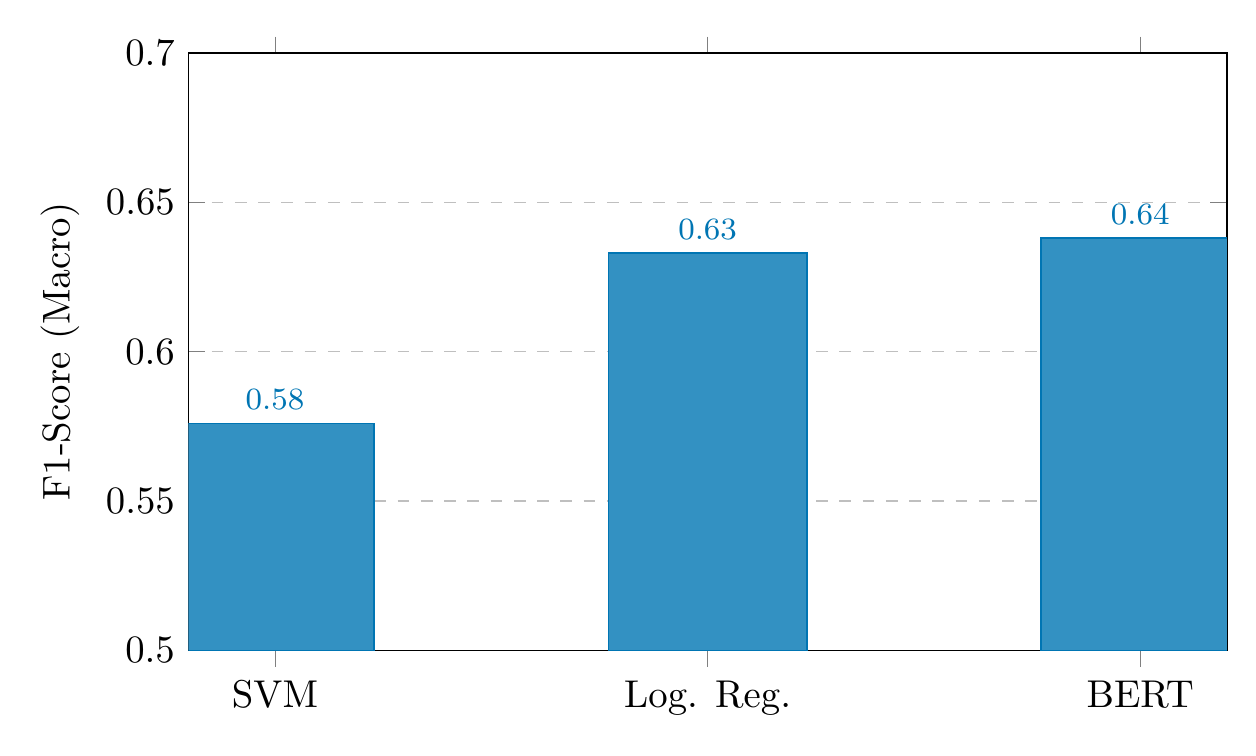
\begin{tikzpicture}[scale=1.4]
\begin{axis}[
  ybar,
  ylabel={F1-Score (Macro)},
  ymajorgrids=true,
  grid style=dashed,
  symbolic x coords={SVM, Log. Reg., BERT},
  xtick=data,
  ymin=0.50,
  ymax=0.70,
  bar width=1.8cm,
  width=11cm,
  height=7cm,
  nodes near coords,
  nodes near coords align={vertical},
  every node near coord/.append style={font=\footnotesize},
]
\addplot[color=hogent-blue, fill=hogent-blue!80] coordinates {
    (SVM, 0.576) 
    (Log. Reg., 0.633) 
    (BERT, 0.638)
};
\end{axis}
\end{tikzpicture}
\vspace{10pt}
\\
\footnotesize \textcolor{html-gray-text}{Figuur 2: Macro F1-score vergelijking per model op de testset}
\end{center}

\vspace{16pt}
\textbf{Invloed inhoudelijke factoren:}\\
Berichtlengte toont het sterkste effect: langere berichten leiden vaker tot classificatiefouten. Lage bronbetrouwbaarheid en specifieke taalkenmerken (woordaantal, vraagtekens) beïnvloeden de nauwkeurigheid tevens significant ($p<0.05$).


\htmlsection{Conclusies \& Discussie}

\begin{itemize}
    \item \textbf{Antwoord op onderzoeksvraag:} BERT presteert allround het best (Macro F1: 0.638). Logistic Regression vormt echter een onverwacht sterke en rekenkundig \textbf{lichtgewicht baseline}. SVM kampt met een sterke bias naar "waar".
    \item \textbf{Praktische implicaties:} Voor het Fediverse, met beperkte middelen per instance, is een \textbf{hybride aanpak} ideaal: lichte modellen (LR) lokaal voor snelle voorselectie, en zware modellen (BERT) voor complexe of twijfelachtige signalen.
    \item \textbf{Wetenschappelijke bijdrage:} Machine learning is effectief in gefragmenteerde decentrale omgevingen. Zowel tekstinhoud als bronmetadata dragen cruciale signalen in zich.
\end{itemize}


\htmlsection{Toekomstig onderzoek}

Multimodale detectie (tekst + beeld via CLIP), Explainable AI (LIME/SHAP) voor betere transparantie richting moderatoren, en de integratie van netwerkkenmerken zoals de defederatie-historiek.

\end{multicols}
\end{document}